\nonstopmode
\documentclass{beamer}
%\documentclass[handout]{beamer}
%\includeonlylecture{week12}



\providecommand{\cpp}{C\kern-0.05em\texttt{+\kern-0.03em+} }
\providecommand{\Cpp}{\cpp}

%\usepackage{pdfpages}
\usepackage[utf8]{inputenc}
\usepackage[T1]{fontenc}
\usepackage{lmodern}
\usepackage{import}
\graphicspath{{../pics}}
%\usepackage{pgf}
%\usepackage{ctable}

\usepackage{listings}%[2000/08/23]
\usepackage{lstlangampl} % syntax file, I added some more keywords like 'display'

%\usepackage{graphicx}
%\usepackage{multicol}

%\usepackage{tikz}

\lstnewenvironment{cplus}
    {\lstset{language=c++,basicstyle=\scriptsize,frame=}}
    {}


\lstnewenvironment{cplus3}
    {\lstset{language=c++,basicstyle=\scriptsize,frame=}}
    {}


\lstnewenvironment{java}
    {\lstset{language=java,basicstyle=\scriptsize,frame=}}
    {}

\lstnewenvironment{java2}
    {\lstset{language=java,basicstyle=\scriptsize}}
    {}

\lstdefinelanguage{Haskell-custom}
{%columns=flexible,
escapeinside={--@}{@--},breaklines=true,breakatwhitespace=true%
language=Haskell,basicstyle=\color{lightblue}\ttfamily,keywordstyle=\ttfamily,%
morekeywords={class,instance,type,newtype,data,where,deriving,import},%
lineskip=-.1\baselineskip,morekeywords={concept,requires,concept_map}}

\lstnewenvironment{hask}[1][\small]{\lstset{language=Haskell-custom,%
    style=numbers,basicstyle=\color{lightblue}#1\ttfamily,keywordstyle=#1\ttfamily,%
    style=bold-keywords,style=frametb}}{}

\providecommand{\haskellinl}[2][\normalsize]{{\lstinline[language=Haskell-custom,%
basicstyle=\color{lightblue}#1\ttfamily,keywordstyle=#1\ttfamily]@#2@}}%

\providecommand{\haskinl}[2][\normalsize]{{\lstinline[language=Haskell-custom,%
basicstyle=\color{lightblue}#1\ttfamily,mathescape=true,keywordstyle=#1\ttfamily]@#2@}}%

\lstdefinestyle{markers}{rangeprefix=\{-\:\ ,%
includerangemarker=false,%
rangesuffix=\ \:-\}}%

\providecommand{\haskellinput}[3][\small]{{\lstinputlisting[language=Haskell-custom,basicstyle=\color{lightblue}#1\ttfamily,keywordstyle=#1\ttfamily,%
style=bold-keywords,style=numbers,style=frametb,style=markers,firstnumber=1,linerange={#3}]{#2}}}

\providecommand{\haskellinputnonumber}[3][\small]{{\lstinputlisting[language=Haskell-custom,basicstyle=\color{lightblue}#1\ttfamily,keywordstyle=#1\ttfamily,%
style=bold-keywords,style=frametb,xleftmargin=8pt,xrightmargin=8pt,style=markers,firstnumber=1,linerange={#3}]{#2}}}



\title[Automated Generation of Unit Tests]{Automated Generation of Unit Tests from UML Activity Diagrams using the AMPL Interface for Constraint Solvers} 
\subtitle[M.Sc. Thesis]{A Master Thesis} 
\author[F. Kurth]{Felix Kurth} 
\day=14
\month=1
\year=2014
\date[Jan 2014]{\today} 

\pgfdeclareimage[height=1.2cm]{STS-logo}{STS-logo}
\logo{\pgfuseimage{STS-logo}}

\begin{document}

\begin{frame}
\titlepage
\end{frame}

\begin{frame}
\frametitle{Outline} 
\tableofcontents  
\end{frame}


\section{Introduction}
\subsection{Motivation}
\begin{frame}
\frametitle{Model--Based Engineering at Airbus Buxtehude}
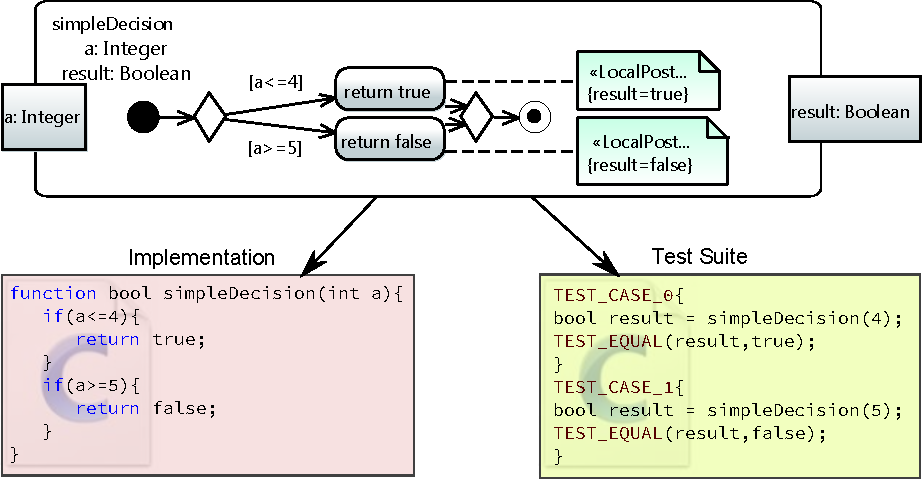
\includegraphics[width=\textwidth]{../Thesis/pics/BasicExamplesSimpleDecision.pdf}
\end{frame}
\subsection{Overview of our Solution}
\begin{frame}
\frametitle{Overview of our Solution}
\begin{description}
\item[Test Model:] A UML activity diagram with embedded OCL constraints modelling an operation/function is used as test model.
\item[Symbolic Execution:] Control flow paths within the activity diagram are executed and stored as constraint satisfaction problem.
\item[Constraint Solving:] A variety of state--of--the--art constraint solvers can be used to generate test data for an executed control flow path.
\item[Language Independent:] Test model and test cases and are stored as an instance of our own intermediate meta models.
\end{description}
\end{frame}


\section{The Algorithm}
\begin{frame}
\frametitle{Overview of the Algorithm}
\begin{block}{Normalisation}
Map UML/OCL to simplified intermediate representation
\end{block}
\begin{block}{Rigorous Mathematical Programming}
Transform activity diagram into an AMPL model
\end{block}
\begin{block}{Abstract Test Case Generation}
Find control flow paths using depth first and breadth first search
\end{block}
\begin{block}{Specific Test Data Generation}
Solve constraint satisfaction problem for each control flow path
\end{block}
\begin{block}{Unit Test Synthesis}
Output test cases as C++ unit tests using the Boost test library
\end{block}
\end{frame}
\subsection{Normalisation}
\begin{frame}
\frametitle{Goals of Normalisation}
\begin{itemize}
  \item Ensure that our algorithm does not run into error conditions
  \item Slice relevant parts out of a huge UML model
  \item Parse embedded OCL constraints and ensure that they comply to the handled OCL subset
  \item Make implicit constraints explicit automatically
\end{itemize}
\begin{block}{}
Subsequent steps are completely independent from the UML/OCL model
\end{block}
\end{frame}
\begin{frame}
\frametitle{The Activity Test Case Graph Model}
	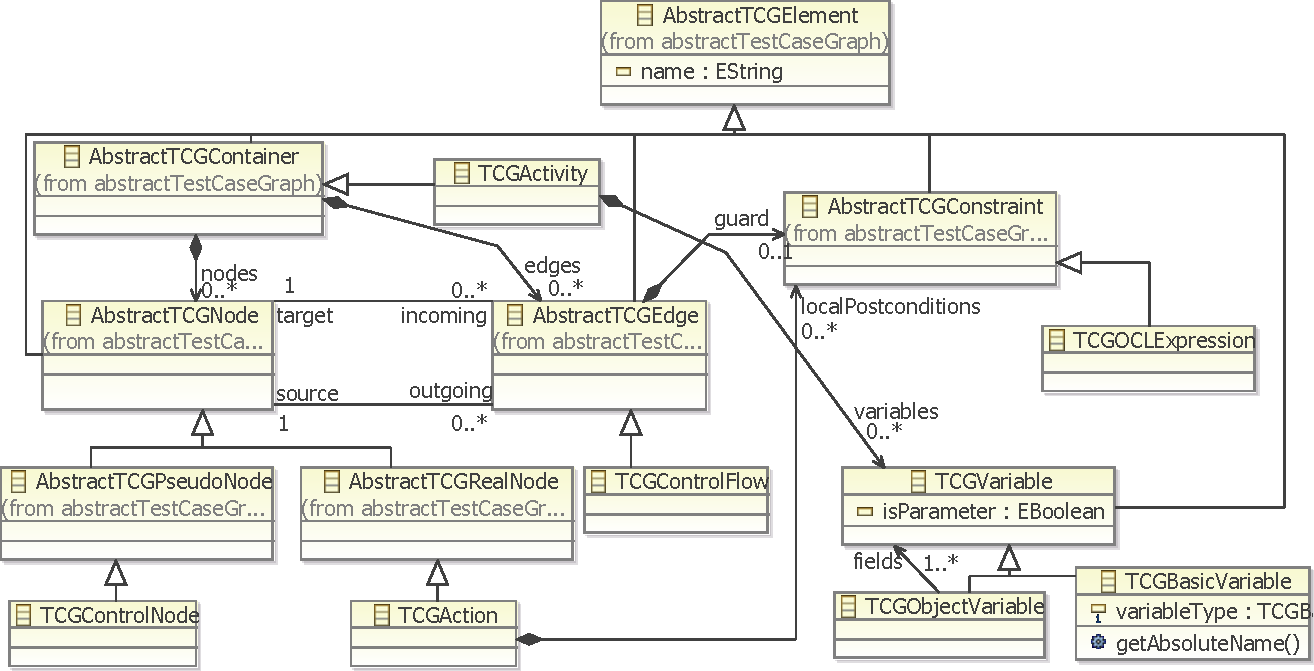
\includegraphics[width=\textwidth]{../IntermediatePresentation/pics/completeMetamodelforSlideshowN.pdf}
\end{frame}

\subsection{Rigorous Mathematical Programming}
\begin{frame}
\frametitle{AMPL Modelling}
\begin{itemize}
  \item Represent activity diagram in a form that is understood by constraint solvers
\end{itemize}
\vspace{0.3cm}
\begin{itemize}
  \item AMPL modelling language\cite{AMPL} allows for transparent exchange of solvers depending on the formulation of constraints
  \item Enable easy encoding of a control flow path as constraint satisfaction problem whose solution is suitable test data
\end{itemize}
% \begin{block}{}
% Represent activity diagram in a form that is understood by constraint solvers
% \end{block}
\end{frame}
\begin{frame}[fragile]
\frametitle{Basic Example}
\begin{columns}
 \column{.39\textwidth} \ 
	\begin{block}{Activity Diagram} 
	\def\svgwidth{\textwidth}
	\scriptsize
	\import{pics/}{BasicExamples.pdf_tex}
	\end{block} 
\column{.56\textwidth} \ 
	\begin{block}{AMPL Model} 
		\begin{lstlisting}[basicstyle=\ttfamily\scriptsize,language=ampl]
param l; #Pathlength

# Variables (Property or Parameter)
var x{0..l} : integer := 1;
var y : integer := 1;

# Postconditions
set t within {0..l} default {};
s.t. t_post0{i in t} : (y)=(x[i-1]);
s.t. t_post1{i in t} : (x[i])=(x[i-1]);
set e within {0..l} default {};
s.t. e_post0{i in e} : (y)=(x[i-1]-100);
s.t. e_post0{i in e} : (x[i])=(x[i-1]);

# Guards
set d2e within {0..l} default {};
s.t. d2e_g{i in d2e} : (x[i])>=(6.0);
set d2t within {0..l} default {};
s.t. d2t_g{i in d2t} : (x[i])<=(5.0);
\end{lstlisting}
	\end{block} 
\end{columns}
\end{frame}

% \begin{frame}[fragile]
% \frametitle{AMPL Modelling}
% 	\begin{block}{Specify Path} 
% 		\begin{lstlisting}[basicstyle=\ttfamily\small,language=ampl]
% param l := 1;
% set d2f:= 0; # guard 
% set f:= 1; # post condition
% 		\end{lstlisting}
% 	\end{block} 
% 	\begin{block}{Result} 
% 		\begin{lstlisting}[basicstyle=\ttfamily\small]
% Solution determined by presolve.
% a = 5
% return = 0
% 		\end{lstlisting}
% 	\end{block}
% \end{frame}

\subsection{Abstract Test Case Generation}
\begin{frame}
\frametitle{Abstract Test Case Generation}
\begin{itemize} 
\item Determine appropriate test scenarios fulfilling model structure based coverage criteria
\item Detect infeasible control flow paths as early as possible
\end{itemize}
\vspace{0.3cm}
\begin{itemize} 
\item Simple breadth first or depth first search used to find control flow paths
\item Maximum path length or a fixed number of control flow paths can be given as parameter to ensure termination of the algorithm
\item Infeasible paths are eliminated by solving all constraints along a path
\item How often infeasible path elimination is performed can be controlled by the parameter unchecked steps
%\item Infeasible paths elimination is performed whenever search is currently examining a real decision node and unchecked steps decision nodes have already been passed without a check
\end{itemize}
\end{frame} 


\subsection{Specific Test Data Generation}

\begin{frame}
\frametitle{Specific Test Data Generation}
\begin{itemize} 
\item For each test scenario input data and oracle values need to be computed
\item Values at the boundaries of path constraints are known to trigger bugs with a higher likelihood
\end{itemize}
\vspace{0.3cm}
\begin{itemize} 
\item Control flow path is symbolically executed and encoded in AMPL data
\item State--of--the--art constraint solver generates test input and the oracle value from the AMPL program
\item Boundary value analysis is possible by adding an objective function to the AMPL model
\item All generated test data is stored in a language independent unit test model
\end{itemize}
\end{frame}

\begin{frame}
\frametitle{Tested Solvers}
\begin{center}
\begin{tabular}{l r r r r r r r r}
Solver & LP & MILP & COP & OP & SAT & SMT & FCSP & MINLP\\
\hline
Cplex & \checkmark & \checkmark & & & & & &\\
IlogCP\cite{ilogcp} & \checkmark & \checkmark & & & \checkmark & \checkmark & \checkmark &\\
GeCoDE\cite{gecode} & & & & &\checkmark & \checkmark & \checkmark &\\
JaCoP & & & & &\checkmark & & \checkmark &\\
Couenne\cite{Belotti09couenne} & \checkmark & \checkmark & \checkmark & \checkmark & & & & \checkmark\\
Gurobi & \checkmark & & \checkmark & & & & &\\
LPsolve\cite{lpsolve} & \checkmark &\checkmark  & & & & & &\\
Minos &\checkmark & &\checkmark & & & & &\\
% conopt & & & & & & & &\\
% knitro & & & & & & & &\\
% snopt & & & & & & & &\\
% xpress & & & & & & & &\\
% bonmin & & & & & & & &\\
% cbc & & & & & & & &\\
% ipopt & & & & & & & &\\
\hline
\end{tabular}\end{center}
\end{frame}

\subsection{Unit Test Synthesis}
\begin{frame}
\frametitle{Unit Test Synthesis}
\begin{itemize} 
\item Output compileable unit test code
\item Support state--of--the--art testing framework
\end{itemize}
\vspace{0.3cm}
\begin{itemize} 
\item Model-to-Text transformation from unit test model and activity test case graph
\item Currently C++ unit tests using the Boost test library are generated
\end{itemize}
\end{frame}

\section{Evaluation}
\subsection{Demo}
% \begin{frame}
% \begin{block}{}
% \begin{center}
% \Huge{Demo!}
% \end{center}
% \end{block}
% \end{frame}

\begin{frame}
\frametitle{Triangle Classificator}
% \def\svgwidth{\textwidth}
% \scriptsize
% \input{./pics/TriangleClasificator.pdf_tex}
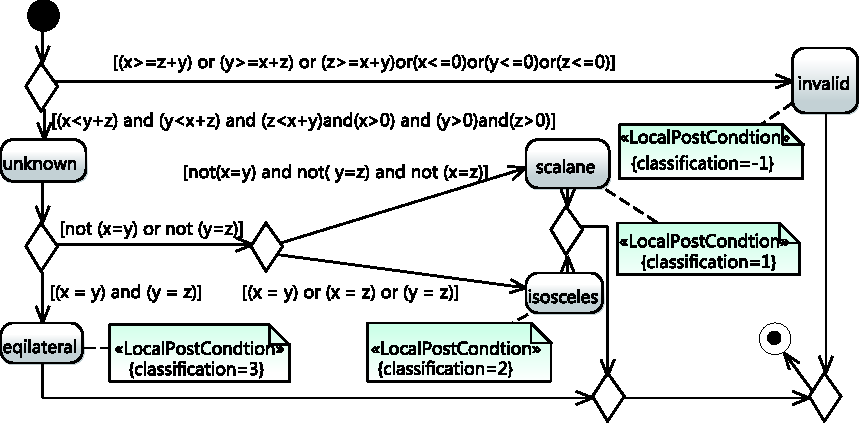
\includegraphics[width=\textwidth]{./pics/TriangleClasivicator.pdf}
\end{frame}
\begin{frame}
\frametitle{Binary Counter}
% \def\svgwidth{\textwidth}
% \scriptsize
% \input{./pics/TriangleClasificator.pdf_tex}
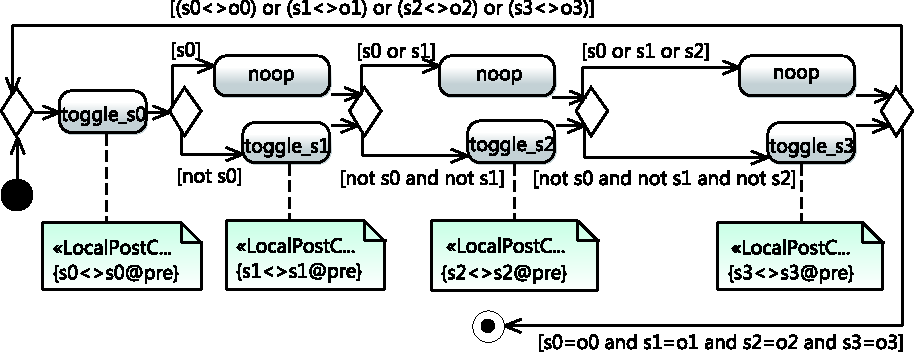
\includegraphics[width=\textwidth]{./pics/BinaryCounderSMT.pdf}
\end{frame}
\begin{frame}
\frametitle{Runtime Measurement for Different Solvers}
\begin{tikzpicture}
\begin{axis}[
width=0.598\textwidth,
height=7.5cm,
xlabel={maximum path length},
ylabel={time $[s]$},
legend style={legend columns=1,at={(0.02,0.98)},anchor=north west},
%yticklabels={0,{$1$},{$10$},{$100$},{$10^3$},{$10^4$},{$10^5$}},
extra y ticks={3.6e12,2.592e14},
extra y tick labels={{1h},{3d}},
extra tick style={
        major grid style=black,
        tick align=outside,
        tick style=black
    },
minor x tick num=1,
ymajorgrids=true,
yminorgrids=true,
xmajorgrids=true,
xminorgrids=true,
ymode=log,
xmin=5,
xmax=95,
]
\addplot[blue,no markers] table[x=PATHSEARCH_MAX_PATHLENGTH,y=time(ns)]{../Thesis/Experiment-DATA/BinaryCounterGecode+presolveSMT.csv};
\addlegendentry{GeCoDE};
\addplot[red,no markers] table[x=PATHSEARCH_MAX_PATHLENGTH,y=time(ns)]{../Thesis/Experiment-DATA/BinaryCounterJacop+presolveSMT.csv};
\addlegendentry{JaCoP};
\end{axis}
\end{tikzpicture}%
\begin{tikzpicture}
\begin{axis}[
width=0.398\textwidth,
height=7.5cm,
nodes near coords,
xmin=5,
xmax=95,
% xtick={10,20,30,40,50,60,70,80,90},
xlabel={maximum path length},
ylabel={total number of test cases},
]
\addplot+[black,mark=x,only marks] table[x=PATHSEARCH_MAX_PATHLENGTH,y=PathsFound]{../Thesis/Experiment-DATA/BinaryCounterGecode+presolveSMT.csv};
\end{axis}
\end{tikzpicture}
\end{frame}

\begin{frame}
\frametitle{Exploding Tyres}
% \def\svgwidth{\textwidth}
% \scriptsize
% \input{./pics/TriangleClasificator.pdf_tex}
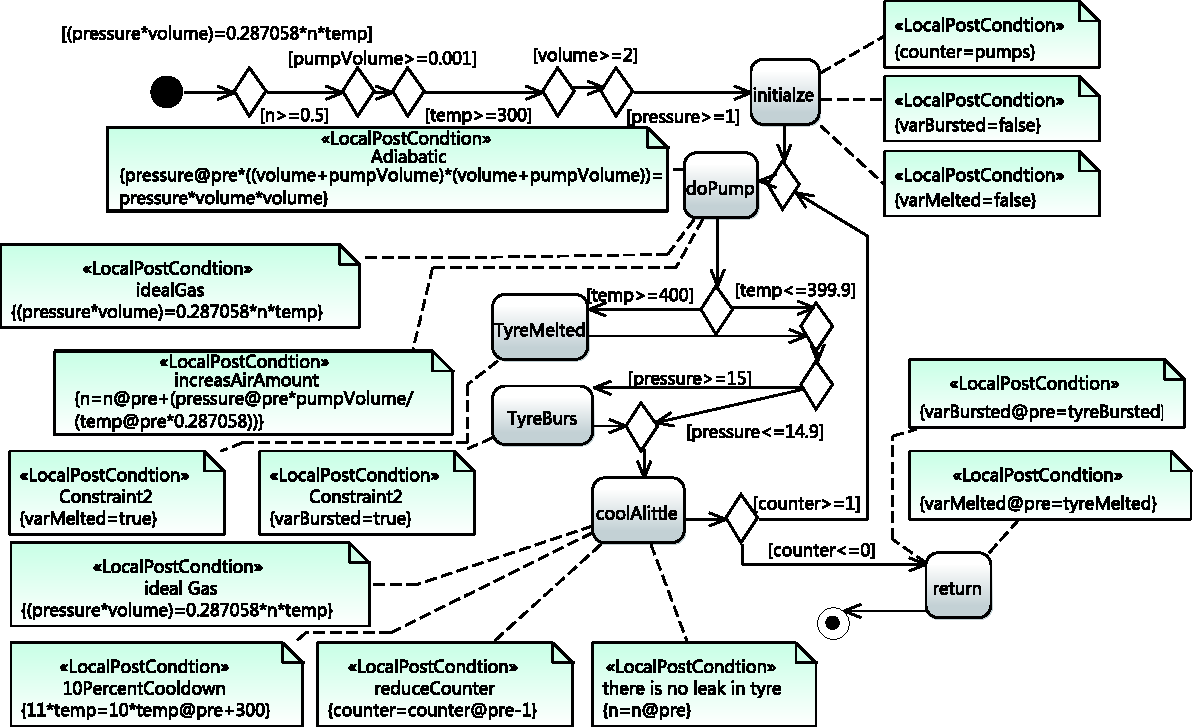
\includegraphics[width=\textwidth]{./pics/TyrePump.pdf}
\end{frame}
\begin{frame}
\frametitle{Runtime Measurement for Different Solver Time Limits}
\begin{tikzpicture}
\begin{axis}[
width=0.498\textwidth,
height=7.5cm,
legend style={legend columns=1,at={(0.02,0.98)},anchor=north west},
% legend to name=myLegend,
ylabel={time $[s]$},
xlabel={maximum path length},
yticklabels={{0},{$0.1$},{$1$},{$10$},{$100$},{$10^3$},{$10^4$},{$10^5$}},
extra y ticks={3.6e12,2.592e14},
extra y tick labels={{1h},{3d}},
extra tick style={
        major grid style=black,
        tick align=outside,
        tick style=black
    },
minor x tick num=1,
ymajorgrids=true,
yminorgrids=true,
xmajorgrids=true,
xminorgrids=true,
ymode=log,
xmin=5,
xmax=75,
]
\addplot[blue,no markers] table[x=PATHSEARCH_MAX_PATHLENGTH,y=time(ns)]{../Thesis/Experiment-DATA/ExplodingTyres_10min.csv};
\addlegendentry{10min};
\addplot[red,no markers] table[x=PATHSEARCH_MAX_PATHLENGTH,y=time(ns)]{../Thesis/Experiment-DATA/ExplodingTyres_20sec.csv};
\addlegendentry{20sec};
\addplot[green,no markers] table[x=PATHSEARCH_MAX_PATHLENGTH,y=time(ns)]{../Thesis/Experiment-DATA/ExplodingTyres_5sec.csv};
\addlegendentry{5sec};
% \addplot[dash pattern=on 7pt off 3pt,no markers] table[x=PATHSEARCH_MAX_PATHLENGTH,y=time(ns)]{../Thesis/Experiment-DATA/ExplodingTyres_10s.csv};
% \addlegendentry{10sec};
% \addplot[loosely dashed,no markers] table[x=PATHSEARCH_MAX_PATHLENGTH,y=time(ns)]{../Thesis/Experiment-DATA/ExplodingTyres_60sec.csv};
% \addlegendentry{60sec};
% \addplot[solid,no markers] table[x=PATHSEARCH_MAX_PATHLENGTH,y=time(ns)]{../Thesis/Experiment-DATA/ExplodingTyres_2h.csv};
% \addlegendentry{2h};
\end{axis}
\end{tikzpicture}%
\begin{tikzpicture}
\begin{axis}[
width=0.498\textwidth,
height=7.5cm,
xlabel={maximum path length},
ylabel={number of test cases found},
minor x tick num=1,
minor y tick num=4,
ymajorgrids=true,
yminorgrids=true,
xmajorgrids=true,
xminorgrids=true,
xmin=35,
xmax=75,
]
\addplot[green,no markers] table[x=PATHSEARCH_MAX_PATHLENGTH,y=PathsFound]{../Thesis/Experiment-DATA/ExplodingTyres_5sec.csv};
%\addlegendentry{5sec};
% \addplot[dash pattern=on 7pt off 3pt,no markers] table[x=PATHSEARCH_MAX_PATHLENGTH,y=PathsFound]{Experiment-DATA/ExplodingTyres_10s.csv};
%\addlegendentry{10sec};
\addplot[red,no markers] table[x=PATHSEARCH_MAX_PATHLENGTH,y=PathsFound]{../Thesis/Experiment-DATA/ExplodingTyres_20sec.csv};
%\addlegendentry{20sec};
% \addplot[loosely dashed,no markers] table[x=PATHSEARCH_MAX_PATHLENGTH,y=PathsFound]{Experiment-DATA/ExplodingTyres_60sec.csv};
%\addlegendentry{60sec};
\addplot[blue,no markers] table[x=PATHSEARCH_MAX_PATHLENGTH,y=PathsFound]{../Thesis/Experiment-DATA/ExplodingTyres_10min.csv};
%\addlegendentry{10min};
\end{axis}
\end{tikzpicture}
\end{frame}
\subsection{Case Study}
\begin{frame}
\frametitle{The Airbus Pax Call Model}
\begin{itemize}
  \item The Original Model
\begin{itemize}
  \item Activity diagram consists of 21 \UMLType{Action}s, 24 \UMLType{ControlNode}s and two nested \UMLType{LoopNode}s
  \item C code snippets are embedded
\end{itemize}
  \item Manual Adaptations
  \begin{itemize}
  \item All variables and C structs are represented by several \UMLType{Property} elements
  \item OCL constraints are deduced with an educated guess from the embedded C code snippets
  \item Hierarchical \UMLType{LoopNode}s are flattened
\end{itemize}
\end{itemize}
\begin{block}{}
The resulting constraint satisfaction problem is a mixed integer linear program
\end{block}
\end{frame}
\begin{frame}
\frametitle{Runtime Depending on the Maximum Path Length}
\begin{tikzpicture}
\begin{axis}[
width=0.59\textwidth,
height=7.5cm,
%legend columns=-1,
%legend to name=solvers,
legend style={at={(0.02,0.98)},anchor=north west},
xlabel={maximum path length},
ylabel={time $[s]$},
yticklabels={0,{$1$},{$10$},{$100$},{$10^3$},{$10^4$},{$10^5$}},
extra y ticks={3.6e12,2.592e14},
extra y tick labels={{1h},{3d}},
extra tick style={
        major grid style=black,
        tick align=outside,
        tick style=black
    },
minor x tick num=1,
xmin=15,
xmax=115,
ymax=1e14,
ymajorgrids=true,
yminorgrids=true,
xmajorgrids=true,
xminorgrids=true,
ymode=log,
]
\addplot[green] table[x=PATHSEARCH_MAX_PATHLENGTH,y=time(ns)] {../Thesis/Experiment-DATA/CaseStudyRuntimeCplex.csv};
\addlegendentry{Cplex};
\addplot[blue] table[x=PATHSEARCH_MAX_PATHLENGTH,y=time(ns)] {../Thesis/Experiment-DATA/CaseStudyRuntimeLPSolve.csv};
\addlegendentry{LPsolve};
\addplot[orange] table[x=PATHSEARCH_MAX_PATHLENGTH,y=time(ns)] {../Thesis/Experiment-DATA/CaseStudyRuntimeCouenne.csv};
\addlegendentry{Couenne};
\addplot[red] table[x=PATHSEARCH_MAX_PATHLENGTH,y=time(ns)] {../Thesis/Experiment-DATA/CaseStudyRuntimeGecode.csv};
\addlegendentry{GeCoDE};
\addplot[dashed] expression[no markers, domain=30:110]{2e7*1.12^(x)} node[pos=0.5,sloped,fill=white, below, opacity=1,text opacity=1] {$1.12 ^ {x}$} ;
\end{axis}
\end{tikzpicture}%
\begin{tikzpicture}
\begin{axis}[
width=0.39\textwidth,
height=7.5cm,
ylabel={number of test cases},
xlabel={maximum path length},
minor x tick num=4,
ymajorgrids=true,
yminorgrids=true,
xmajorgrids=true,
xminorgrids=true,
ymode=log,
]
\addplot[blue] table[x=PATHSEARCH_MAX_PATHLENGTH,y=PathsFound]{../Thesis/Experiment-DATA/CaseStudyRuntimeLPSolve.csv};
\addplot[color=black, style=dashed] expression[no markers, domain=30:100]{1.1 ^ (x)} 
node[pos=0.5,sloped,fill=white, below, opacity=1,text opacity=1] {$1.1 ^ {x}$}
;
\end{axis}
\end{tikzpicture}
\end{frame}
\begin{frame}
\frametitle{Runtime Depending on the Unchecked Steps}
\begin{tikzpicture}
\begin{axis}[
width=0.6\textwidth,
height=7.5cm,
legend style={legend columns=1,at={(1.02,0.98)},anchor=north west},
xlabel={unchecked steps},
xmax=15,
ylabel={time $[s]$},
yticklabels={{$1$},{$10$},{$100$},{$10^3$},{$10^4$},{$10^5$}},
extra y ticks={3.6e12,2.592e14},
extra y tick labels={{1h},{3d}},
extra tick style={
        major grid style=black,
        tick align=outside,
        tick style=black
    },
minor x tick num=1,
ymajorgrids=true,
yminorgrids=true,
xmajorgrids=true,
xminorgrids=true,
ymode=log,
]
\addlegendimage{empty legend}
\addlegendentry{maximum path length}
\addplot[densely dashed, blue] table[x=PATHSEARCH_UNCHECKED_STEPS,y=time(ns)]{../Thesis/Experiment-DATA/CaseStudyUncheckedSteps90.csv};
\addlegendentry{90};
\addplot[densely dashed, green] table[x=PATHSEARCH_UNCHECKED_STEPS,y=time(ns)]{../Thesis/Experiment-DATA/CaseStudyUncheckedSteps80.csv};
\addlegendentry{80};
\addplot[densely dashed, red] table[x=PATHSEARCH_UNCHECKED_STEPS,y=time(ns);]{../Thesis/Experiment-DATA/CaseStudyUncheckedSteps70.csv};
\addlegendentry{70};
\addplot[blue] table[x=PATHSEARCH_UNCHECKED_STEPS,y=time(ns);]{../Thesis/Experiment-DATA/CaseStudyUncheckedSteps60.csv};
\addlegendentry{60};
\addplot[green] table[x=PATHSEARCH_UNCHECKED_STEPS,y=time(ns)]{../Thesis/Experiment-DATA/CaseStudyUncheckedSteps50.csv};
\addlegendentry{50};
\addplot[red] table[x=PATHSEARCH_UNCHECKED_STEPS,y={time(ns)}]{../Thesis/Experiment-DATA/CaseStudyUncheckedSteps40.csv};
\addlegendentry{40};
\end{axis}
\end{tikzpicture}
\end{frame}
\begin{frame}
\frametitle{Runtime Depending on the Number of Test Cases}
\begin{tikzpicture}
\begin{axis}[
width=\textwidth,
height=7.5cm,
legend style={legend columns=1,at={(0.02,0.98)},anchor=north west},
xlabel={number of test cases},
ylabel={time $[s]$},
scaled y ticks = false,
% xtick scale label code/.code={\xdef\xtickscale{#1}}, 
yticklabels={0,{$1$},{$10$},{$100$},{$10^3$},{$10^4$},{$10^5$}},
extra y ticks={3.6e12,2.592e14},
extra y tick labels={{1h},{3d}},
extra tick style={
        major grid style=black,
        tick align=outside,
        tick style=black
    },
minor x tick num=1,
ymajorgrids=true,
yminorgrids=true,
xmajorgrids=true,
xminorgrids=true,
ymode=log,
xmode=log,
] 
\addplot[red] table[x=PathsFound,y=time(ns)]{../Thesis/Experiment-DATA/CaseStudyRuntimeBFS.csv};
\addlegendentry{breadth first search (Cplex)}
\addplot[green] table[x=PathsFound,y=time(ns)]{../Thesis/Experiment-DATA/CaseStudyRuntimeCplex.csv};
\addlegendentry{depth first search (Cplex)}
\addplot[blue] table[x=PathsFound,y=time(ns)]{../Thesis/Experiment-DATA/CaseStudyRuntimeLPSolve.csv};
\addlegendentry{depth first search (LPSolve)}
\addplot[color=black, style=dashed] expression[no markers, domain=1e2:1e5]{(2e7) * x}
node [pos=0.7,below,sloped,fill=white,opacity=0.85,text opacity=1] {$x^1$} 
;
\addplot[color=black, style=dashed] expression[no markers, domain=1e2:1e5]{(4e6) * x ^ (1.45)} 
node [pos=0.9,sloped,above,fill=white,opacity=0.85,text opacity=1] {$x^{1.45}$} 
;
\addplot[color=black, style=dashed] expression[no markers, domain=1e2:1e4]{(6e5) * x ^ (2)} 
node [pos=0.7,sloped,above,fill=white,opacity=0.85,text opacity=1] {$x^{2}$} 
;
\end{axis}
\end{tikzpicture}%
% \begin{tikzpicture}
% \begin{axis}[
% width=0.49\textwidth,
% height=7.5cm,
% xlabel={number of test cases},
% ylabel={time $[s]$},
% scaled y ticks = false,
% % xtick scale label code/.code={\xdef\xtickscale{#1}}, 
% %xtick scale label code/.code={$10^3$}, 
% %xtick scale label code/.code={\xdef\xtickscale{#1}},
% yticklabels={{0},{0},{$2\cdot 10^{3}$},{ },{$6\cdot 10^{3}$},{$8\cdot 10^{3}$}},
% extra y ticks={3.6e12,2.592e14},
% extra y tick labels={{1h},{3d}},
% extra tick style={
%         major grid style=black,
%         tick align=outside,
%         tick style=black
%     },
% minor x tick num=1,
% minor y tick num=4,
% ymajorgrids=true,
% yminorgrids=true,
% xmajorgrids=true,
% xminorgrids=true,
% xmin=500,
% xmax=9500,
% ] 
% \addplot[blue] table[x=PathsFound,y=time(ns)]{../Thesis/Experiment-DATA/CaseStudyRuntimeCplex.csv};
% \addlegendentry{depth first search}
% \addplot[red] table[x=PathsFound,y=time(ns)]{../Thesis/Experiment-DATA/CaseStudyRuntimeBFS.csv};
% \addlegendentry{breadth first search}
% \end{axis}
% \end{tikzpicture}%
\end{frame}
\begin{frame}
\frametitle{Runtime with and without Boundary Value Analysis}
\begin{tikzpicture}
\begin{axis}[
width=\textwidth,
height=7.5cm,
%title={Influence of boundary value analysis},
legend style={at={(0.02,0.98)},anchor=north west},
ylabel={time $[s]$},
xlabel={maximum path length},
%ytick={1e8,1e10,1e12,1e14},
yticklabels={0,{1},{10},{100},{$10^3$},{$10^4$},{$10^5$}},
extra y ticks={3.6e12,2.592e14},
extra y tick labels={{1h},{3d}},
extra tick style={
        major grid style=black,
        tick align=outside,
        tick style=black
    },
ymajorgrids=true,
yminorgrids=true,
xmajorgrids=true,
xminorgrids=true,
ymode=log,
]
\addplot[blue] table[x=PATHSEARCH_MAX_PATHLENGTH,y=time(ns)]{../Thesis/Experiment-DATA/CaseStudyRuntimeBoundaryValues.csv};
\addlegendentry{with};
\addplot[red] table[x=PATHSEARCH_MAX_PATHLENGTH,y=time(ns)]{../Thesis/Experiment-DATA/CaseStudyRuntimeNoBoundaryValues.csv};
\addlegendentry{without}
\end{axis}
\end{tikzpicture}%
\end{frame}

\section{Summary}
\begin{frame}
\frametitle{Summary}
\begin{itemize}
  \item In general there are very little restrictions on the formulation of constraints, but mixed integer linear programming can be handled especially efficiently
  \item All control flow paths is not a feasible coverage criterion, the Abstract Test Case Generation should be improved accordingly
  \item This approach can easily be adapted to other input models (other UML Tools) and other output languages due to its internal model representation
\end{itemize}
\end{frame}

\section*{Appendix}
\begin{frame}
\begin{block}{Thank you!}
\begin{center}
\Huge{Questions?}
\end{center}
\end{block}
\end{frame}
\frametitle{Bibliography}
\bibliographystyle{IEEEtran}
%\bibliographystyle{plain}
\bibliography{../Thesis/bibtex}
\end{document}
